%% abtex2-modelo-relatorio-tecnico.tex, v-1.9.2 laurocesar
%% Copyright 2012-2014 by abnTeX2 group at http://abntex2.googlecode.com/ 
%%
%% This work may be distributed and/or modified under the
%% conditions of the LaTeX Project Public License, either version 1.3
%% of this license or (at your option) any later version.
%% The latest version of this license is in
%%   http://www.latex-project.org/lppl.txt
%% and version 1.3 or later is part of all distributions of LaTeX
%% version 2005/12/01 or later.
%%
%% This work has the LPPL maintenance status `maintained'.
%% 
%% The Current Maintainer of this work is the abnTeX2 team, led
%% by Lauro César Araujo. Further information are available on 
%% http://abntex2.googlecode.com/
%%
%% This work consists of the files abntex2-modelo-relatorio-tecnico.tex,
%% abntex2-modelo-include-comandos and abntex2-modelo-references.bib
%%

% ------------------------------------------------------------------------
% ------------------------------------------------------------------------
% abnTeX2: Modelo de Relatório Técnico/Acadêmico em conformidade com 
% ABNT NBR 10719:2011 Informação e documentação - Relatório técnico e/ou
% científico - Apresentação
% ------------------------------------------------------------------------ 
% ------------------------------------------------------------------------

\documentclass[
	% -- opções da classe memoir --
	12pt,				% tamanho da fonte
	openright,			% capítulos começam em pág ímpar (insere página vazia caso preciso)
	oneside,			% para impressão em verso e anverso. Oposto a oneside
	a4paper,			% taman
	ho do papel. 
	% -- opções da classe abntex2 --
	%chapter=TITLE,		% títulos de capítulos convertidos em letras maiúsculas
	%section=TITLE,		% títulos de seções convertidos em letras maiúsculas
	%subsection=TITLE,	% títulos de subseções convertidos em letras maiúsculas
	%subsubsection=TITLE,% títulos de subsubseções convertidos em letras maiúsculas
	% -- opções do pacote babel --
	english,			% idioma adicional para hifenização
	french,				% idioma adicional para hifenização
	spanish,			% idioma adicional para hifenização
	brazil,				% o último idioma é o principal do documento
	]{abntex2}

% ---
% Pacotes básicos 
% ---
\usepackage{lmodern}
% Usa a fonte Latin Modern	

\usepackage[T1]{fontenc}
%\hyphenation{ ir-re-ver-s\'{i}-veis}
\hyphenation{co-nhe-ci-men-to a-pre-sen-ta-do}
% Selecao de codigos de fonte.
\usepackage[utf8]{inputenc}			% Codificacao do documento (conversão automática dos acentos)
\usepackage{lastpage}				% Usado pela Ficha catalográfica
\usepackage{indentfirst}			% Indenta o primeiro parágrafo de cada seção.
\usepackage{color}					% Controle das cores
\usepackage{graphicx}				% Inclusão de gráficos e imagens
\usepackage{microtype} 				% para melhorias de justificação
\usepackage{mathtools}				% Matemática
\usepackage{multirow}				% Tabelas
\usepackage[table,xcdraw]{xcolor}	% Tabelas (cores)
% ---
\usepackage{float}
\usepackage{gensymb}

\usepackage{amssymb}
\usepackage{subcaption}
\usepackage[utf8]{inputenc}
\usepackage[export]{adjustbox}
\usepackage{wrapfig}
\usepackage{amsmath}
\usepackage{mathtools}
\usepackage{pdfpages}
\usepackage{subfiles}


\graphicspath{{figs/}}

\hyphenpenalty=10000
		
% ---
% Pacotes adicionais, usados apenas no âmbito do Modelo Canônico do abnteX2
% ---
\usepackage{lipsum}				% para geração de dummy text
% ---

% ---
% Pacotes de citações
% ---
\usepackage[brazilian,hyperpageref]{backref}	 % Paginas com as citações na bibl
%\usepackage[alf]{abntex2cite}	% Citações padrão ABNT
\usepackage[alf,abnt-etal-list=0]{abntex2cite}

\usepackage{tabularx}

\newcommand{\otoprule}{\midrule[\heavyrulewidth]}
\usepackage{color,soul}
\usepackage[nomargin,inline]{fixme}
\fxusetheme{color}
\fxsetup{draft}
% \fxsetup{final}
\FXRegisterAuthor{prc}{pm}{\color{red}Paulo}
\FXRegisterAuthor{cls}{cs}{\color{red}Salles}
% --- 
% CONFIGURAÇÕES DE PACOTES
% --- 

% ---
% Configurações do pacote backref
% Usado sem a opção hyperpageref de backref
\renewcommand{\backrefpagesname}{Citado na(s) página(s):~}
% Texto padrão antes do número das páginas
\renewcommand{\backref}{}
% Define os textos da citação
\renewcommand*{\backrefalt}[4]{
	\ifcase #1 %
		Nenhuma citação no texto.%
	\or
		Citado na página #2.%
	\else
		Citado #1 vezes nas páginas #2.%
	\fi}%
% ---

% ---
% Informações de dados para CAPA e FOLHA DE ROSTO
% ---
\titulo{Autoria Multimídia com Uso de Realidade Aumentada}
\autor{Paulo Renato Conceição Mendes}
\local{São Luís - MA}
\data{2019}
\orientador{Prof. Dr. Carlos de Salles Soares Neto}
\tipotrabalho{Monografia (Graduação)}
% O preambulo deve conter o tipo do trabalho, o objetivo, 
% o nome da instituição e a área de concentração 
\preambulo{Monografia apresentada ao curso de Ciência da Computação da Universidade Federal do Maranhão como parte dos requisitos necessários para obtenção do grau de Bacharel em Ciência da Computação.}
% ---


% ---
% Configurações de aparência do PDF final

% alterando o aspecto da cor azul
\definecolor{blue}{RGB}{41,5,195}

% informações do PDF
\makeatletter
\hypersetup{
     	%pagebackref=true,
		pdftitle={\@title}, 
		pdfauthor={\@author},
    	pdfsubject={\imprimirpreambulo},
	    pdfcreator={LaTeX with abnTeX2},
		pdfkeywords={abnt}{latex}{abntex}{abntex2}{trabalho acadêmico}, 
		colorlinks=true,       		% false: boxed links; true: colored links
    	linkcolor=blue,          	% color of internal links
    	citecolor=blue,        		% color of links to bibliography
    	filecolor=magenta,      		% color of file links
		urlcolor=blue,
		bookmarksdepth=4
}
\makeatother
% --- 

% --- 
% Espaçamentos entre linhas e parágrafos 
% --- 

% O tamanho do parágrafo é dado por:
\setlength{\parindent}{1.3cm}

% Controle do espaçamento entre um parágrafo e outro:
\setlength{\parskip}{0.2cm}  % tente também \onelineskip

% ---
% compila o indice
% ---
\makeindex
% ---

% ----
% Início do documento
% ----
\begin{document}

% Seleciona o idioma do documento (conforme pacotes do babel)
%\selectlanguage{english}
\selectlanguage{brazil}

% Retira espaço extra obsoleto entre as frases.
\frenchspacing 

% ----------------------------------------------------------
% ELEMENTOS PRÉ-TEXTUAIS
% ----------------------------------------------------------
% \pretextual

% ---
% Capa
% ---
\imprimircapa
% ---CDU 
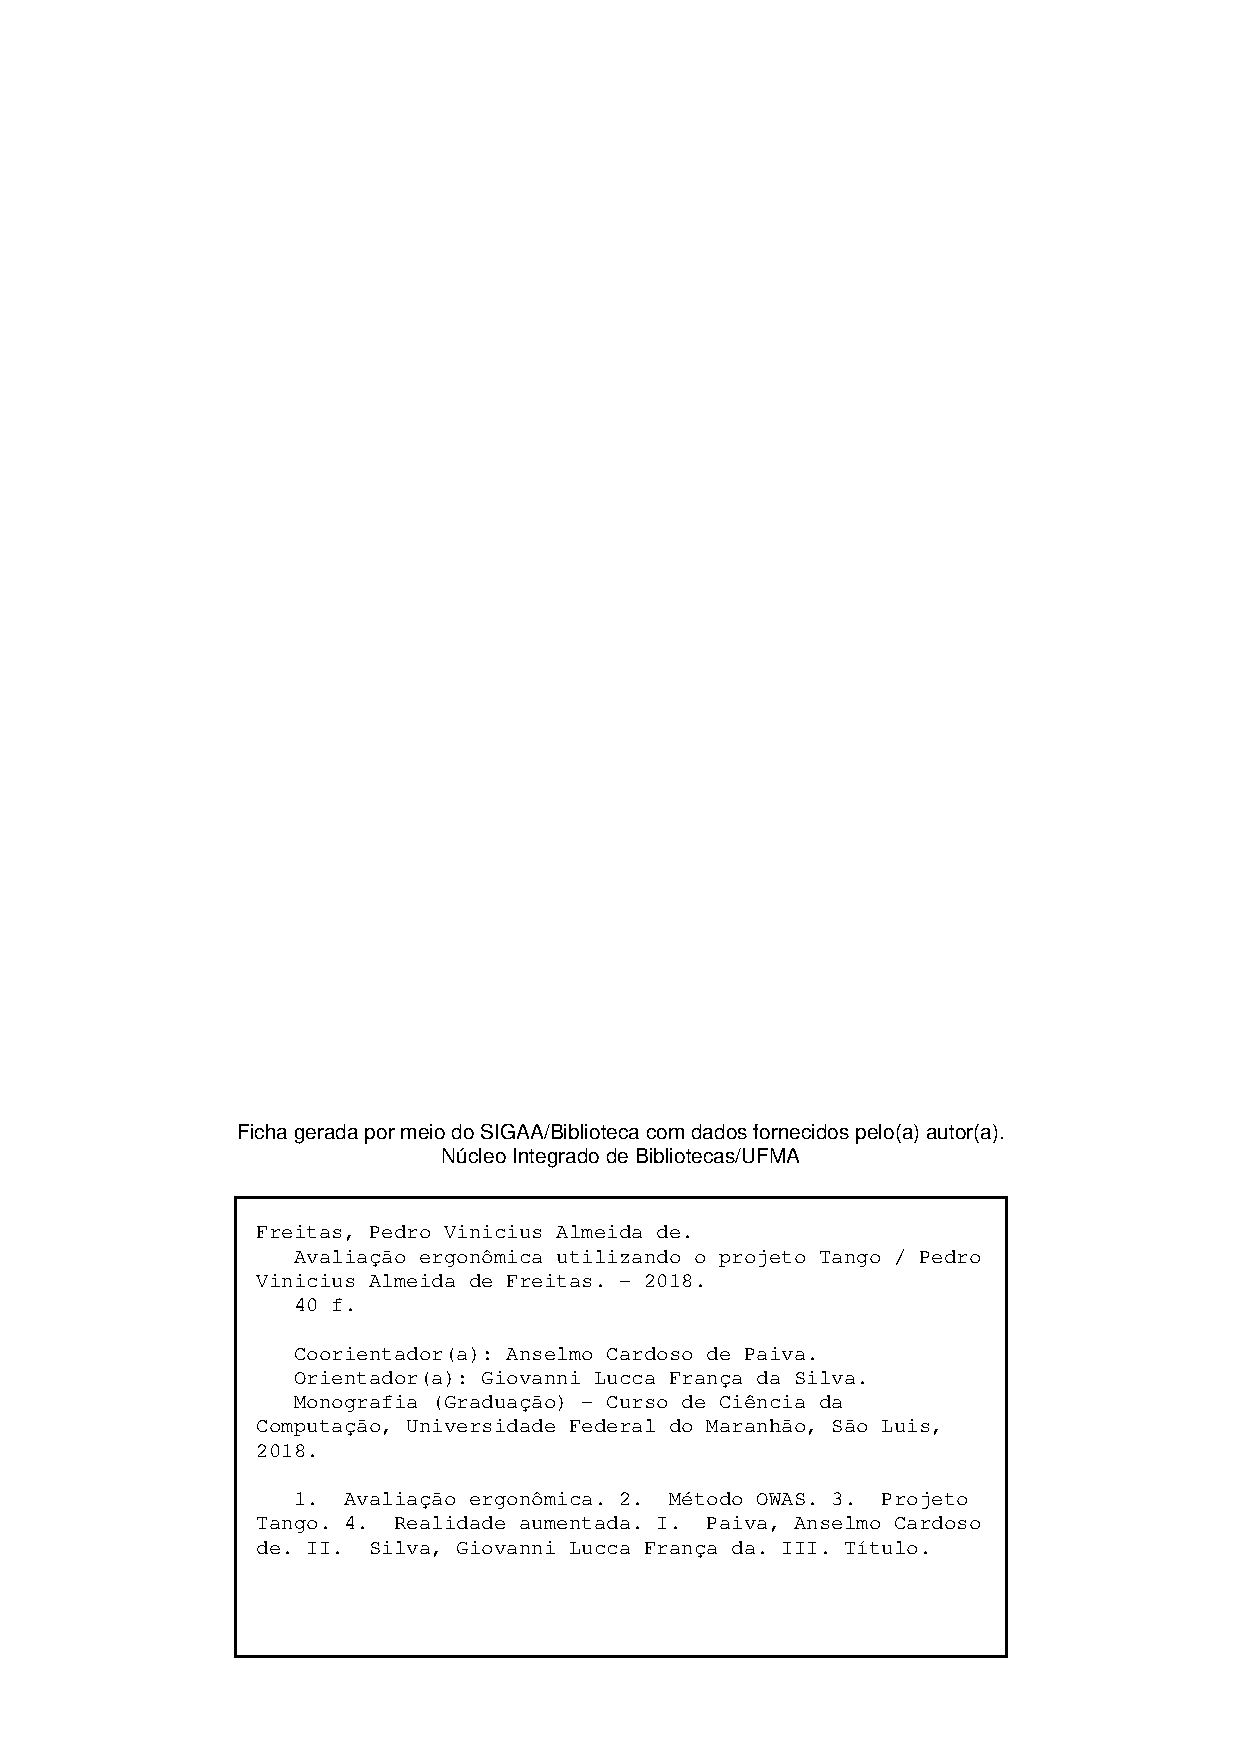
\includepdf{ficha.pdf}
% ---
% Folha de rosto
% (o * indica que haverá a ficha bibliográfica)
% ---
%\imprimirfolhaderosto
\iffalse
\begin{folhadeaprovacao}


 	\begin{center}
 		{\ABNTEXchapterfont\large\imprimirautor} \\
         \vspace{1cm} 
 		{\ABNTEXchapterfont\Large\bfseries\imprimirtitulo}
 	\end{center}
   \vspace{1cm} 
   \hspace{.45\textwidth} 
   \begin{minipage}{.5\textwidth} 
   \imprimirpreambulo \vspace{1cm} 
 	\end{minipage} 
 	\vspace{1cm}  \\
 	Trabalho aprovado em 27 de junho de 2019:
      %\imprimirlocal, \imprimirdata: 
 %%%%%%%%%%%%%%%%%%%%%%%%%%%%%%%%%%%%%%%%%%%%%%%% 
 %Assinaturas 
% %%%%%%%%%%%%%%%%%%%%%%%%%%%%%%%%%%%%%%%%%%%%%% 
 \assinatura{\imprimirorientador \\ Orientador \\ Universidade Federal do Maranhão } 


 \assinatura{Prof. Dr. Mário Antonio Meireles Teixeira\\Examinador\\Universidade Federal do Maranhão} 
 \assinatura{Prof. Dr. Anselmo Cardoso de Paiva\\ Examinador\\ Universidade Federal do Maranhão} 

% %%%%%%%%%%%%%%%%%%%%%%%%%%%%%%%%%%%%%%%%%%%%%%%%%% 
% % 
% %%%%%%%%%%%%%%%%%%%%%%%%%%%%%%%%%%%%%%%%%%%%%%%%%%% 
 \begin{center} 
 \vfill 
 {\large\imprimirlocal} 
 \par 
 {\large\imprimirdata} 
 \end{center} 
 \end{folhadeaprovacao} 
\fi
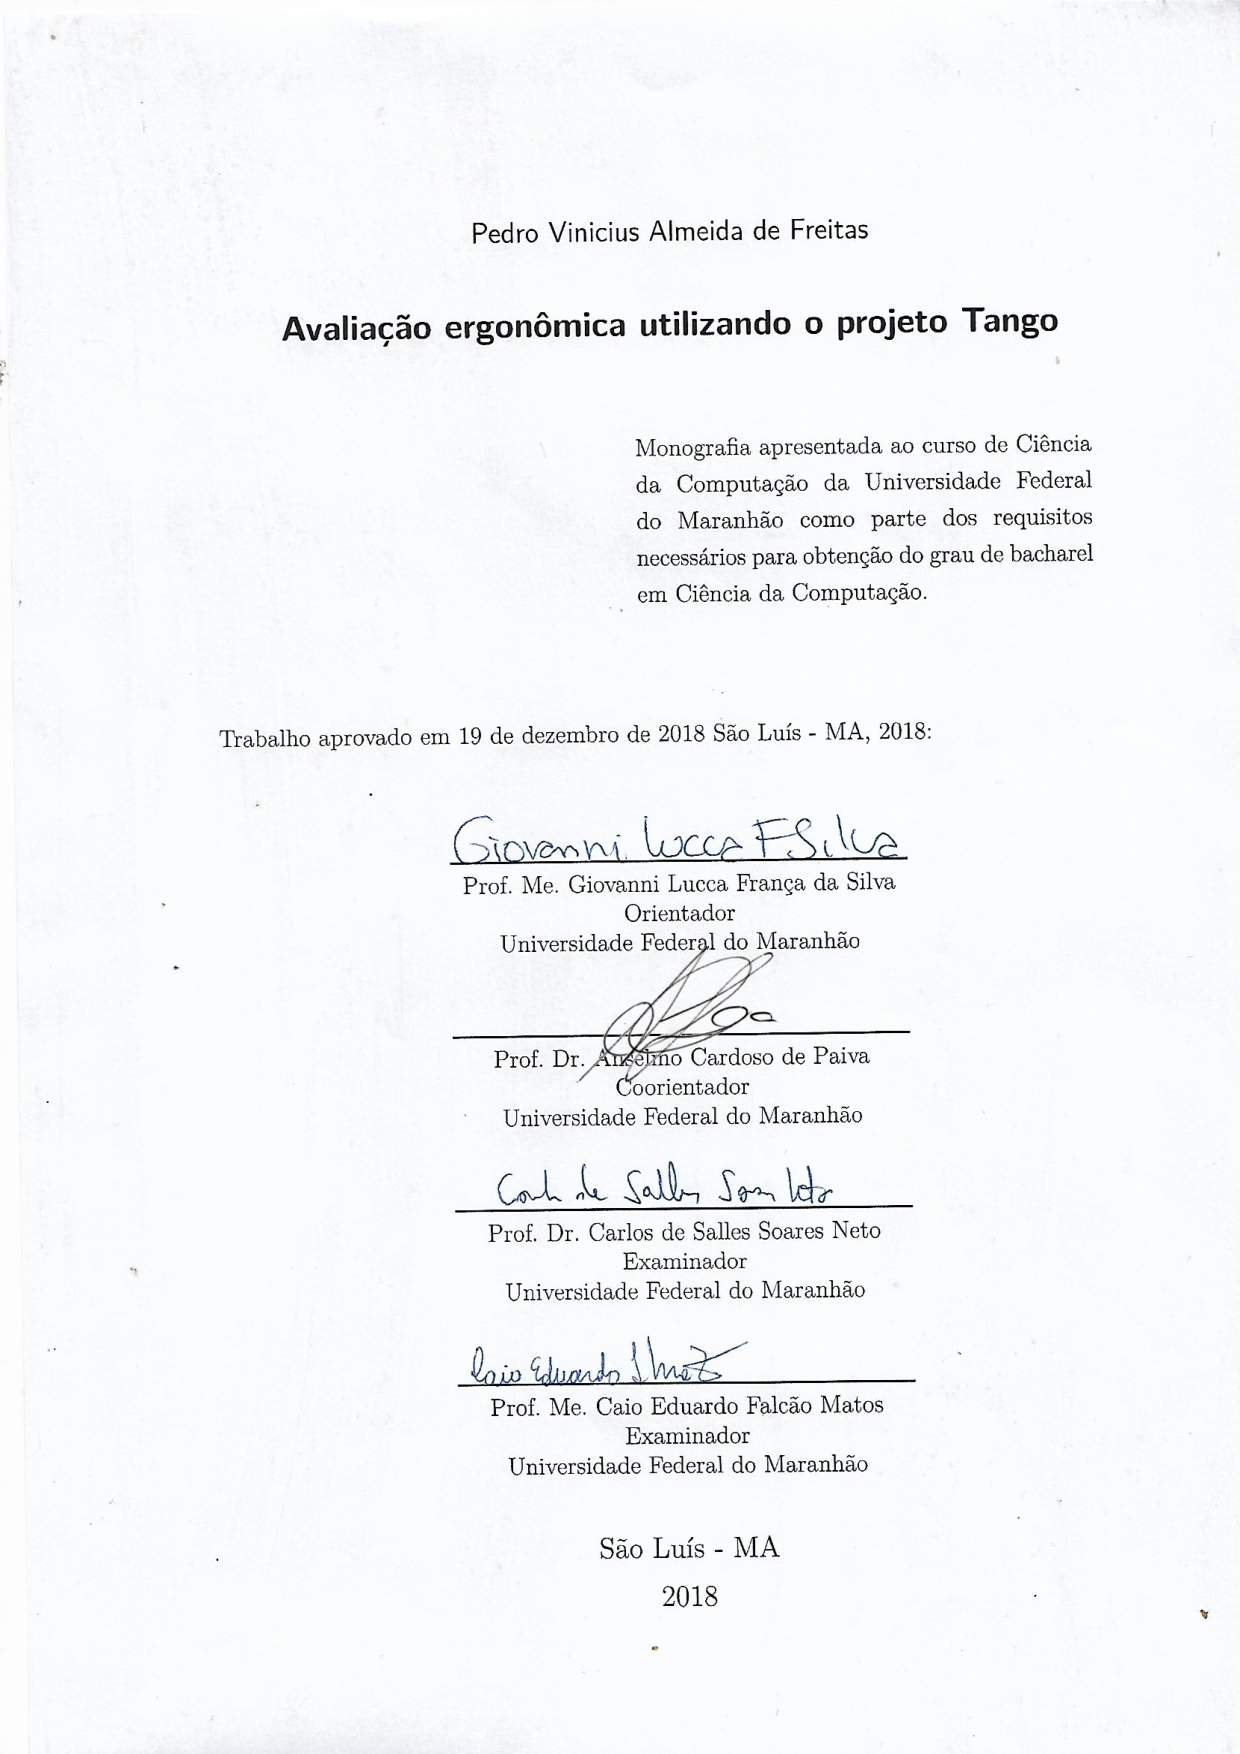
\includepdf{assinaturas.pdf}

%%%%%%%%%%%%%%%%%%%%%%%%%%%%%%%%% 
% Início da dedicatória - Elemento opcional 
%%%%%%%%%%%%%%%%%%%%%%%%%%%%%%%%%%%%%%%%%%%%%%%%%%%%%%%%%%% 
\begin{dedicatoria} 
\vspace{\fill} 
\begin{center} 
À minha família e meus amigos.
\end{center}
\vspace{\fill} 
\end{dedicatoria} 
%%%%%%%%%%%%%%%%%%%%%%%%%%%%%%%%%%%%%%%%%%%%%%%%%% 
% Fim da dedicatória 
%%%%%%%%%%%%%%%%%%%%%%%%%%%%%%%%%%%%%%%%%%%%%%%%%%


% ---
% Anverso da folha de rosto:
% ---



%\ABNTEXchapterfont

%\vspace*{\fill}

%Conforme a ABNT NBR 10719:2011, seção 4.2.1.1.1, o anverso da folha de rosto
%deve conter:
%
% \begin{alineas}
%  \item nome do órgão ou entidade responsável que solicitou ou gerou o
%   relatório; 
%  \item título do projeto, programa ou plano que o relatório está relacionado;
%  \item título do relatório;
%  \item subtítulo, se houver, deve ser precedido de dois pontos, evidenciando a
%   sua subordinação ao título. O relatório em vários volumes deve ter um título
%   geral. Além deste, cada volume pode ter um título específico; 
%  \item número do volume, se houver mais de um, deve constar em cada folha de
%   rosto a especificação do respectivo volume, em algarismo arábico; 
%  \item código de identificação, se houver, recomenda-se que seja formado
%   pela sigla da instituição, indicação da categoria do relatório, data,
%   indicação do assunto e número sequencial do relatório na série; 
%  \item classificação de segurança. Todos os órgãos, privados ou públicos, que
%   desenvolvam pesquisa de interesse nacional de conteúdo sigiloso, devem
%    informar a classificação adequada, conforme a legislação em vigor; 
%  \item nome do autor ou autor-entidade. O título e a qualificação ou a função
%   do autor podem ser incluídos, pois servem para indicar sua autoridade no
%   assunto. Caso a instituição que solicitou o relatório seja a mesma que o
%   gerou, suprime-se o nome da instituição no campo de autoria; 
%  \item local (cidade) da instituição responsável e/ou solicitante; NOTA: No
%   caso de cidades homônimas, recomenda-se o acréscimo da sigla da unidade da
%   federação.
%  \item ano de publicação, de acordo com o calendário universal (gregoriano),
%  deve ser apresentado em algarismos arábicos.
% \end{alineas}

%\vspace*{\fill}
%}

% ---
% Agradecimentos
% ---
\begin{agradecimentos}

Aos meus pais, Antonio e Dulce, por me ensinaram desde cedo sobre o poder transformador da educação, pelo apoio de sempre e por me guiarem durante toda a minha formação.

À minha irmã, Nicole, pelo incentivo de sempre mesmo eu a irritando constantemente.

Ao meu orientador, Carlos de Salles, pelos conselhos, orientações, conversas e apoio desde o começo do curso.

Aos professores Simara, Ari, Anselmo, Geraldo, Giovanni, Dallyson e todos os demais professores que contribuiram para a minha formação.

A Ninguém (Pedro Almeida), por ser o companheiro de todas as horas e grande parceiro nessa jornada acadêmica.

A Erik e Robert, pelas caronas e amizade.

A Luciano, pelas conversas e conselhos.

A Ylderlan, por ser um grande exemplo de esforço e dedicação.

A Polyana, pela amizade e conselhos acadêmicos e não acadêmicos.

A Anderson Silva, por ser um grande amigo desde o ensino médio.

A todos os demais amigos do codebuilders, companheiros nessa jornada de conhecimento e memes.

A Lucas, Daniel, Ruy e todos os demais amigos e parceiros do Telemídia-MA.

A Kelson, Ricardo, Arthur, Eduardo e todos os demais colegas do LabPai.

A Roberto Gerson, por sua ajuda e orientação na condução deste trabalho.

A Fabiana Moura, cujo apoio foi decisivo para o alcance que este trabalho obteve.

A Márcio Moreno e Jack Jansen, cujos comentários ajudaram a evoluir este trabalho.

À FAPEMA, pelo apoio financeiro a este trabalho.



\end{agradecimentos}

%%%%%%%%%%%%%%%%%%%%%%% 
% Início da epígrafe - opcional 
%%%%%%%%%%%%%%%%%%%%%%%%%%%%%%%%%%%%%%%%%%%%%%%%%%%%%%%%%%%%%% 
\begin{epigrafe} 
\vspace*{\fill} 
\begin{flushright} 
\textit{"São as nossas escolhas, mais do que as nossas capacidades, que mostram quem realmente somos."} 

\textit{(Alvo Dumbledore)}
\end{flushright} 


\end{epigrafe} 
%%%%%%%%%%%%%%%%%%%%%%%%%%%%%%%%%%%%%%%%%%%%%%%%%%%%%%%%%%%%%%%%% 
% Fim da epígrafe - opcional 
%%%%%%%%%%%%%%%%%%%%%%%%%%%%%%%%%%%%%%%%%%%%%%%%%%%%%%%%%%%%%%

% ---

% ---
% RESUMO
% ---

% resumo na língua vernácula (obrigatório)
%\setlength{\absparsep}{18pt} % ajusta o espaçamento dos parágrafos do resumo
\begin{resumo}

Este trabalho apresenta a BumbAR, uma abordagem baseada em realidade aumentada para a autoria de apresentações multimídia, e avalia tal abordagem por meio de um estudo qualitativo baseado no modelo TAM. A abordagem BumbAR é baseada no modelo NCM e explora o uso de realidade aumentada e objetos do mundo real (marcadores) como uma forma inovadora de interface com o usuário para descrever os comportamentos e relações entre objetos de mídia presentes na apresentação. Tal abordagem é concretizada na ferramenta BumbAR, que a implementa. O estudo qualitativo teve o objetivo de avaliar a atitude dos usuários em relação ao uso da BumbAR. Os resultados mostraram que os participantes consideram que a abordagem proposta é útil e fácil de usar, enquanto a maioria deles consideram que o sistema é mais conveniente do que ferramentas de autoria tradicionais. Os comentários dos participantes do estudo mostraram a necessidade da inclusão de novas funcionalidades na ferramenta. 

\noindent
\textbf{Palavras-chave}: Realidade aumentada, multimídia, ferramenta de autoria, interface de usuário.

\end{resumo}

% resumo em inglês
% \include{estrutura/resumo_en}
\begin{resumo}[Abstract]
\begin{otherlanguage*}{english}

This work presents BumbAR, an approach based on augmented reality for authoring multimedia presentations and evaluate it through a qualitative study based on the TAM model. The BumbAR approach is based on the NCM model and explores the use of augmented reality and real-world objects (markers) as an innovative user interface for describing the behavior and relationships between the media objects that are part of a multimedia presentation. The proposed approach is concretized in the BumbAR tool, which implements it. The qualitative study aimed at evaluating users' attitude towards using BumbAR. The results showed that the participants found that the proposed approach is both useful and easy-to-use, while most of them found the system more convenient than traditional desktop-based authoring tools. Comments made by the participants showed the need of including new funcionalities in the BumbAR tool.

\noindent
\textbf{Keywords}: Augmented reality, multimedia, authoring tool, user interface.
\end{otherlanguage*}
\end{resumo}
% ---
\cleardoublepage
% ---
% inserir lista de ilustrações
% ---
\pdfbookmark[0]{\listfigurename}{lof}
\listoffigures*
\cleardoublepage
% ---

% ---
% inserir lista de tabelas
% ---
\pdfbookmark[0]{\listtablename}{lot}
\listoftables*
\cleardoublepage
% ---

% ---
% inserir lista de abreviaturas e siglas
% ---
\begin{siglas}
    %\item[AACR] American Association for Cancer Research

  \item[GUI] Graphical User Interface
  \item[HTML] Hypertext Markup Language
  \item[IHC] Interação Humano Computador
  \item[NCL] Nested Context Language  
  \item[NCM] Nested Context Model  
  \item[PEOU] Perceived Ease-of-use
  \item[POI] Points of Interest    
  \item[PU] Perceived Usefulness
  \item[RA] Realidade Aumentada
  \item[RV] Realidade Virtual  
  \item[SMIL] Synchronized Multimedia Language  
  \item[TAM] Technology Acceptance Model
  \item[TUI] Tangible User Interface
  \item[URL] Uniform Resource Locator
  
  
  
\end{siglas}
% ---

% ---
% inserir lista de símbolos
% ---
%\begin{simbolos}
%  \item[$ \in $] Pertence
%\end{simbolos}
% ---

% ---
% inserir o sumario
% ---
\pdfbookmark[0]{\contentsname}{toc}
\tableofcontents*
\cleardoublepage
% ---


% ----------------------------------------------------------
% ELEMENTOS TEXTUAIS
% ----------------------------------------------------------
\textual

\subfile{Chapters/Introducao.tex} 

\subfile{Chapters/Relacionados.tex} 

\subfile{Chapters/Proposta.tex} 

\subfile{Chapters/Avaliacao.tex} 

\subfile{Chapters/Conclusoes.tex} 

\postextual

% ----------------------------------------------------------
% Referências bibliográficas
% ----------------------------------------------------------
\bibliography{main.bib}
\end{document}